\chapter{Implementation, Integration and Test Plan}

The application is based on three logical layers (data, logic and presentation) that can be implemented in parallel.\\
The whole system can be tested in parallel following a bottom-up approach (see later), this is due to the fact that all the components can be developed independently and then integrated together, and so the testing can be done in an incremental way to evaluate the dependencies between the subcomponents.

\section{Development plan}
Since the front-end relies on APIs provided by the back-end, we will focus more on the back-end development, in order to provide the front-end developers with the APIs they need.

\subsection{Front-end}
Even if it relies on the back-end APIs, the front-end can be developed in parallel with the back-end, since the APIs are well defined and documented; it is sufficient to provide a mock-up of the json objects that will be returned by the APIs to correctly develop the front-end.

\subsection{Back-end}
As said before, the back-end development is the most important part of the project, since it provides the front-end with the APIs it needs.\\
The order of the development of the subcomponents is given by the dependencies between them, so the order is the following:

\begin{enumerate}
    \item \textbf{DBMS}: it is the core of the data layer, so it is the first component to be developed. It includes the implementation of the e-r diagram given in Figure \ref{fig:er_diagram}
    \item \textbf{Query manager}: it is the component that provides the APIs to the logic layer that will be used to query the database. It is the second component to be developed since it relies on the DBMS and it is the only component that can access the database.
    \item \textbf{Auth manager, Notification manager}: they shall be implemetnted before the other subcomponents because they are used by the other subcomponents to authenticate the users and to send notifications to them. Since they are independent from each other, they can be developed in parallel.
    \item \textbf{All other subcomponents}: they can be developed in parallel since they are sufficiently independent from each other. If, for any reason, a subcomponent needs to interact with another one, it can see the other one as a black box
\end{enumerate}

\section{Integration plan}
Now it is shown the order in which the subcomponents will be integrated together to form the whole system.\\
Each component will be uint tested before being integrated with the other components, and after the integration the whole component will be tested.\\
The order of the integration is given by the dependencies between the subcomponents, so the order is shown by the following graphs (for the sake of simplicity, the graphs show only the dependencies between the subcomponents omitting the interfaces between them):\\

The first component to be integrated is the DBMS, since it is the core of the data layer.\\

\begin{figure}[H]
    \centering
    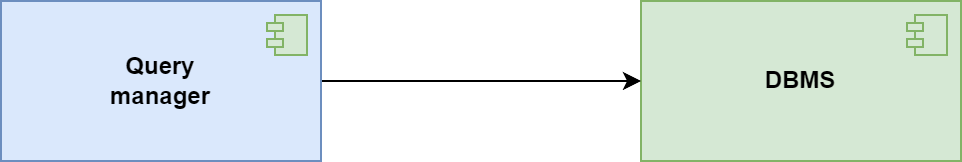
\includegraphics[width=0.6\textwidth]{images/test_plan/test-plan-1.png}
    \caption{Integration plan for the data layer}
    \label{fig:test-plan-1}
\end{figure}

The second component to be integrated is the auth manager, since it makes all the system behave differently based on the user's permissions and so we need to ensure that the auth manager works correctly before integrating the other components (especially, to ensure that the query to the databases are done by an authenticated user at the right level).\\

\begin{figure}[H]
    \centering
    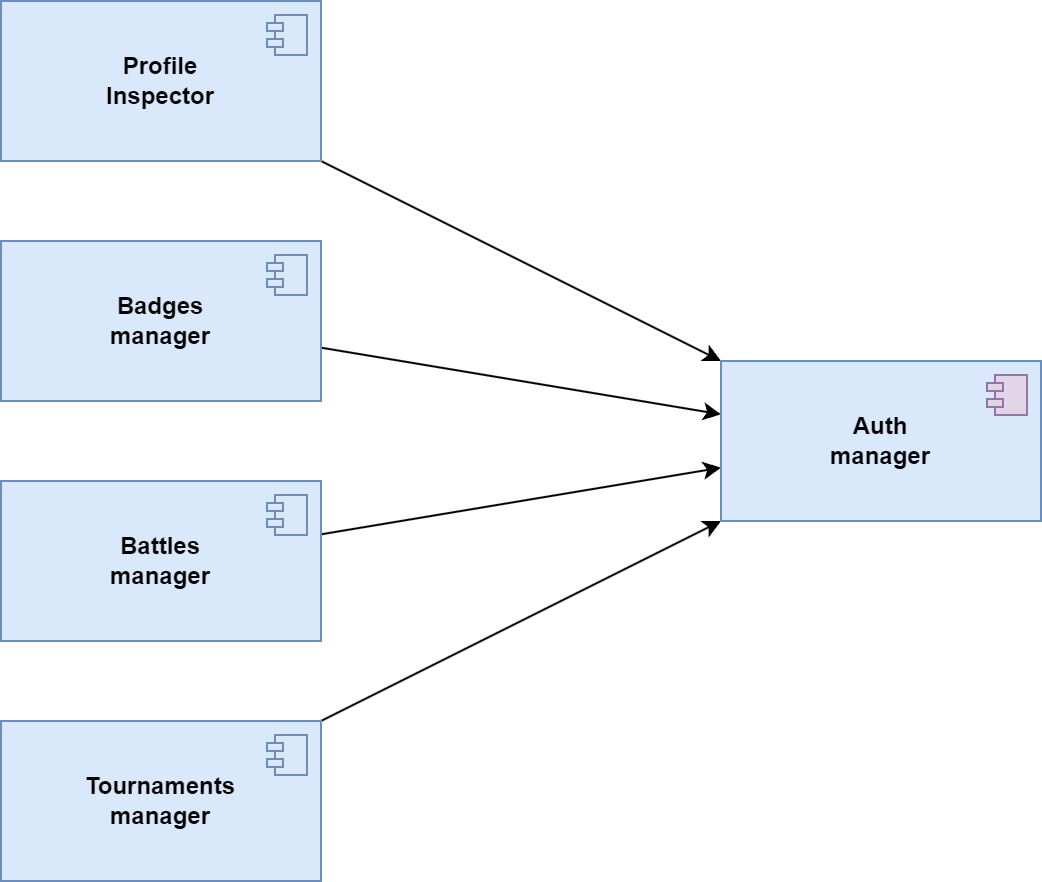
\includegraphics[width=0.6\textwidth]{images/test_plan/test-plan-2.png}
    \caption{Integration plan for the auth manager}
    \label{fig:test-plan-2}
\end{figure}

The third component to be integrated is the query manager, since it is the only component that can access the database and nearly all the other components rely on it to query the database.\\

\begin{figure}[H]
    \centering
    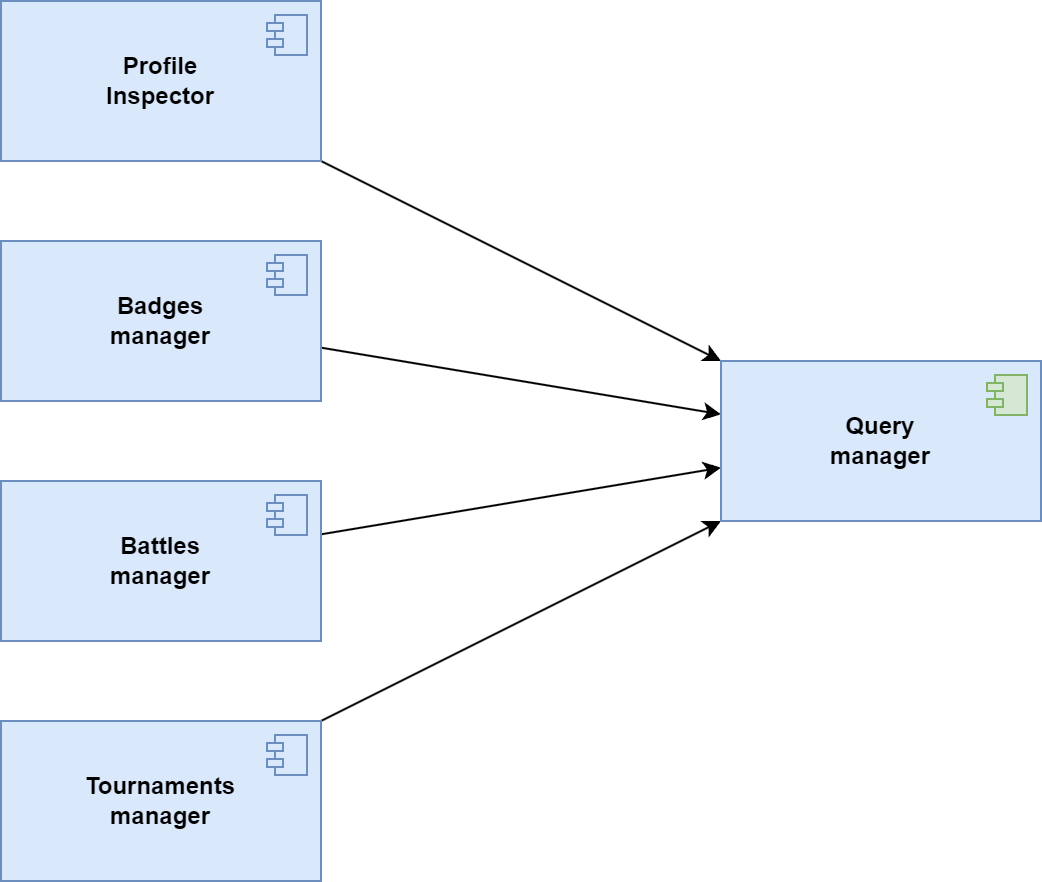
\includegraphics[width=0.6\textwidth]{images/test_plan/test-plan-3.png}
    \caption{Integration plan for the query manager}
    \label{fig:test-plan-3}
\end{figure}

Another component that needs to be integrated is the notification manager, since it is used by the other components to send notifications to the users.\\
It can be integrated in parallel with the other Query Manager, since it does not need to access the database, the notifications to be sent are provided by the other components.\\

\begin{figure}[H]
    \centering
    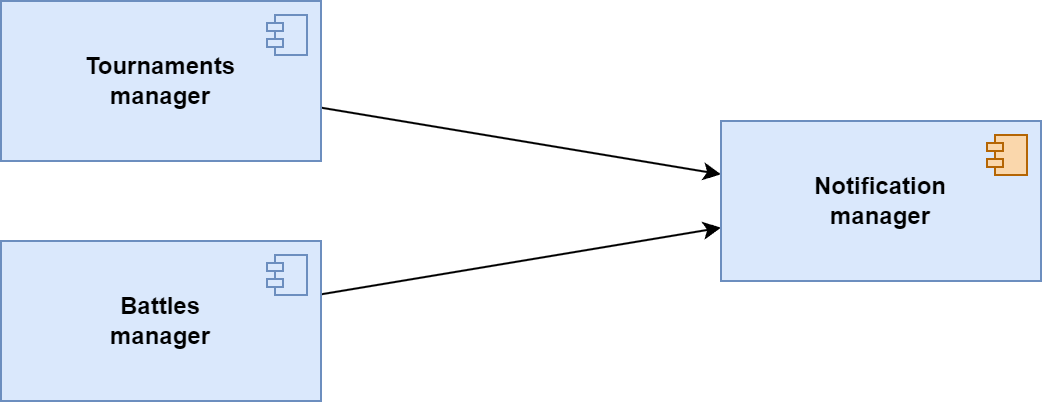
\includegraphics[width=0.6\textwidth]{images/test_plan/test-plan-4.png}
    \caption{Integration plan for the notification manager}
    \label{fig:test-plan-4}
\end{figure}

Finally, once all the unit tests are passed and the components are integrated together, the presentation layer can be integrated with the other components and a full testing phase can be performed on the whole system.\\

\begin{figure}[H]
    \centering
    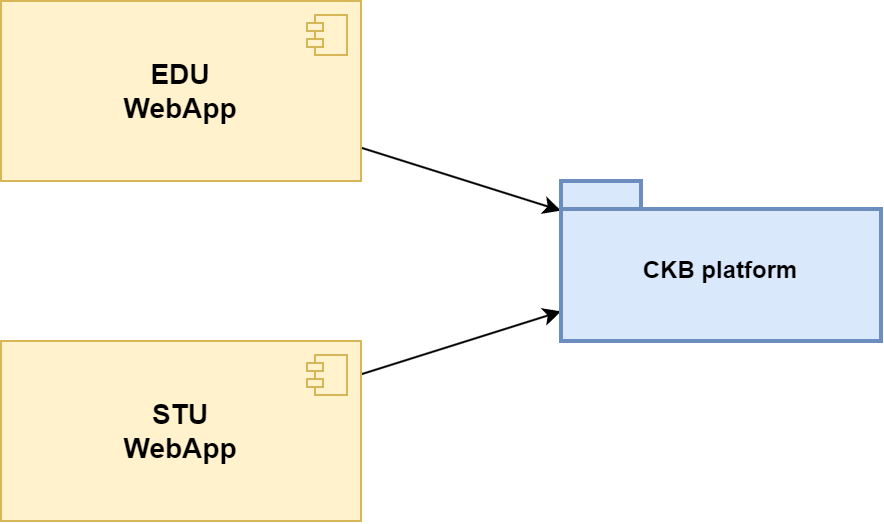
\includegraphics[width=0.6\textwidth]{images/test_plan/test-plan-5.png}
    \caption{Integration plan for the presentation layer}
    \label{fig:test-plan-5}
\end{figure}

The aim of the testing phase is to verify the functional and non-functional requirements and must take place in a testing environment that is as close as possible to the production environment.\\
To ensure the minimum probability of failure of the released software, two kinds of testing will be performed:

\begin{itemize}
    \item \textbf{functional testing}: it will be performed to verify that the system meets the functional requirements, in particular, the ones specified on the RASD document.
    \item \textbf{performance testing}: it will be performed to verify that the system meets the non-functional requirements, in particular, wether the software remains functional with increase demand and various environment conditions.
\end{itemize}